% called by main.tex
% Vinh
\chapter{Kết quả mô phỏng}
\label{ch::chapter3}

Phần mô phỏng được thực hiện với các kích thước gói tin khác nhau, bao gồm 4 gói tin với kích thước lần lượt là 8kb, 16kb, 40kb và 80kb. Số trạm (Station hoặc Node) sử dụng trong mô phỏng là từ 10 đến 400.
Có 5 chiến lược (Strategy) được mô phỏng bao gồm:
\begin{itemize}
    \item Strategy 1: Tăng CW = CW * 2 khi xảy ra xung đột và đặt lại CW = CWmin khi truyền dữ liệu thành công.
    \item Strategy 2: Tăng CW = CW + 2 khi xảy ra xung đột và giữ nguyên CW khi truyền dữ liệu thành công.
    \item Strategy 3: Tăng CW = CW * 2 khi xảy ra xung đột và giữ nguyên CW khi truyền dữ liệu thành công.
    \item Strategy 4: Tăng CW = CW + 2 khi xảy ra xung đột và giảm CW = CW - 2 khi truyền dữ liệu thành công.
    \item Strategy 5: Tăng CW = CW * 2 khi xảy ra xung đột và giảm CW = CW - 2 khi truyền dữ liệu thành công.
\end{itemize}

Từ các kết quả mô phỏng trong hình~\ref{fig:result}, ta có thể rút ra kết luận như sau:
\begin{itemize}
    \item Với Packet\_size = 8kb: kết quả mô phỏng cho thấy: cả Strategy 1,2,3,4,5 đều có hiệu suất tốt (trên 50\%) và có thể thấy Strategy 3,5 là tốt nhất.
    \item Với Packet\_size = 16kb: cả Strategy 1,2,3,4,5 đều có hiệu suất tốt (trên 50\%) và có thể thấy Strategy 3,5 là tốt nhất.
    \item Với Packet\_size = 40kb: kết quả mô phỏng lúc này khi ta càng nâng cao Packet\_size thì hiệu suất của các Strategy sẽ càng giảm đối với các Strategy 1,3,5 hiểu suất giảm so với Packet\_size = 40kb chỉ trong khoảng 10\% còn Strategy 2,4 hiệu suất bị giảm đến 30\%.
    \item Với Packet\_size = 80kb: so với Packet\_size = 40000 các Strategy 1,2,3,4,5 có hiệu suất giảm đi khoảng 10\%.
\end{itemize}

\begin{figure}[h]
    \centering
    \begin{subfigure}{0.45\linewidth}
        % This file was created by matlab2tikz.
%
%The latest updates can be retrieved from
%  http://www.mathworks.com/matlabcentral/fileexchange/22022-matlab2tikz-matlab2tikz
%where you can also make suggestions and rate matlab2tikz.
%
\definecolor{mycolor1}{rgb}{0.00000,0.44700,0.74100}%
\definecolor{mycolor2}{rgb}{0.85000,0.32500,0.09800}%
\definecolor{mycolor3}{rgb}{0.92900,0.69400,0.12500}%
\definecolor{mycolor4}{rgb}{0.49400,0.18400,0.55600}%
\definecolor{mycolor5}{rgb}{0.46600,0.67400,0.18800}%
%
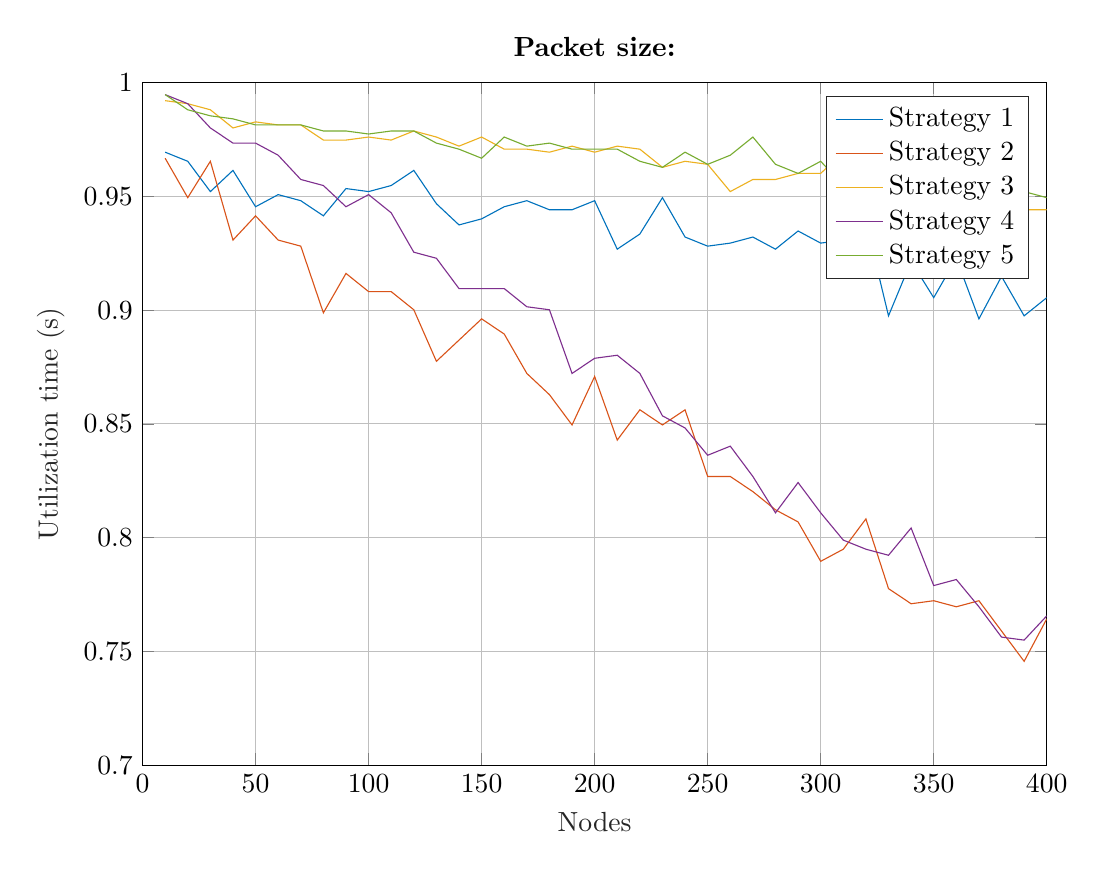
\begin{tikzpicture}

\begin{axis}[%
width=4.521in,
height=3.414in,
at={(0.758in,0.481in)},
scale only axis,
xmin=0,
xmax=400,
xlabel style={font=\color{white!15!black}},
xlabel={Nodes},
ymin=0.7,
ymax=1,
ylabel style={font=\color{white!15!black}},
ylabel={Utilization time (s)},
axis background/.style={fill=white},
title style={font=\bfseries},
title={Packet size:},
xmajorgrids,
ymajorgrids,
legend style={legend cell align=left, align=left, draw=white!15!black}
]
\addplot [color=mycolor1]
  table[row sep=crcr]{%
10	0.969374167776299\\
20	0.96537949400799\\
30	0.952063914780294\\
40	0.961384820239681\\
50	0.945406125166446\\
60	0.950732356857524\\
70	0.948069241011985\\
80	0.941411451398137\\
90	0.953395472703063\\
100	0.952063914780294\\
110	0.954727030625833\\
120	0.961384820239681\\
130	0.946737683089215\\
140	0.937416777629828\\
150	0.940079893475367\\
160	0.945406125166446\\
170	0.948069241011985\\
180	0.944074567243676\\
190	0.944074567243676\\
200	0.948069241011985\\
210	0.926764314247671\\
220	0.933422103861519\\
230	0.949400798934754\\
240	0.932090545938749\\
250	0.928095872170441\\
260	0.92942743009321\\
270	0.932090545938749\\
280	0.926764314247671\\
290	0.934753661784289\\
300	0.92942743009321\\
310	0.93075898801598\\
320	0.938748335552598\\
330	0.897470039946739\\
340	0.921438082556593\\
350	0.905459387483357\\
360	0.922769640479362\\
370	0.89613848202397\\
380	0.914780292942744\\
390	0.897470039946739\\
400	0.905459387483357\\
};
\addlegendentry{Strategy 1}

\addplot [color=mycolor2]
  table[row sep=crcr]{%
10	0.96671105193076\\
20	0.949400798934754\\
30	0.96537949400799\\
40	0.93075898801598\\
50	0.941411451398137\\
60	0.93075898801598\\
70	0.928095872170441\\
80	0.898801597869509\\
90	0.916111850865514\\
100	0.908122503328896\\
110	0.908122503328896\\
120	0.900133155792279\\
130	0.877496671105195\\
140	0.886817576564582\\
150	0.89613848202397\\
160	0.889480692410122\\
170	0.872170439414117\\
180	0.862849533954729\\
190	0.849533954727033\\
200	0.870838881491347\\
210	0.842876165113185\\
220	0.856191744340881\\
230	0.849533954727033\\
240	0.856191744340881\\
250	0.82689747003995\\
260	0.82689747003995\\
270	0.820239680426102\\
280	0.812250332889484\\
290	0.806924101198405\\
300	0.7896138482024\\
310	0.794940079893479\\
320	0.808255659121175\\
330	0.777629826897474\\
340	0.770972037283626\\
350	0.772303595206395\\
360	0.769640479360856\\
370	0.772303595206395\\
380	0.758988015978699\\
390	0.745672436751003\\
400	0.764314247669778\\
};
\addlegendentry{Strategy 2}

\addplot [color=mycolor3]
  table[row sep=crcr]{%
10	0.992010652463382\\
20	0.990679094540613\\
30	0.988015978695073\\
40	0.980026631158456\\
50	0.982689747003995\\
60	0.981358189081225\\
70	0.981358189081225\\
80	0.974700399467377\\
90	0.974700399467377\\
100	0.976031957390147\\
110	0.974700399467377\\
120	0.978695073235686\\
130	0.976031957390147\\
140	0.972037283621838\\
150	0.976031957390147\\
160	0.970705725699068\\
170	0.970705725699068\\
180	0.969374167776299\\
190	0.972037283621838\\
200	0.969374167776299\\
210	0.972037283621838\\
220	0.970705725699068\\
230	0.962716378162451\\
240	0.96537949400799\\
250	0.96404793608522\\
260	0.952063914780294\\
270	0.957390146471372\\
280	0.957390146471372\\
290	0.960053262316911\\
300	0.960053262316911\\
310	0.969374167776299\\
320	0.956058588548603\\
330	0.950732356857524\\
340	0.956058588548603\\
350	0.953395472703063\\
360	0.949400798934754\\
370	0.958721704394142\\
380	0.942743009320906\\
390	0.944074567243676\\
400	0.944074567243676\\
};
\addlegendentry{Strategy 3}

\addplot [color=mycolor4]
  table[row sep=crcr]{%
10	0.994673768308922\\
20	0.990679094540613\\
30	0.980026631158456\\
40	0.973368841544608\\
50	0.973368841544608\\
60	0.968042609853529\\
70	0.957390146471372\\
80	0.954727030625833\\
90	0.945406125166446\\
100	0.950732356857524\\
110	0.942743009320906\\
120	0.925432756324901\\
130	0.922769640479362\\
140	0.909454061251666\\
150	0.909454061251666\\
160	0.909454061251666\\
170	0.901464713715048\\
180	0.900133155792279\\
190	0.872170439414117\\
200	0.878828229027965\\
210	0.880159786950734\\
220	0.872170439414117\\
230	0.853528628495342\\
240	0.848202396804263\\
250	0.836218375499337\\
260	0.840213049267646\\
270	0.82689747003995\\
280	0.810918774966714\\
290	0.82423435419441\\
300	0.810918774966714\\
310	0.798934753661788\\
320	0.794940079893479\\
330	0.79227696404794\\
340	0.804260985352866\\
350	0.778961384820243\\
360	0.781624500665783\\
370	0.769640479360856\\
380	0.75632490013316\\
390	0.75499334221039\\
400	0.765645805592547\\
};
\addlegendentry{Strategy 4}

\addplot [color=mycolor5]
  table[row sep=crcr]{%
10	0.994673768308922\\
20	0.988015978695073\\
30	0.985352862849534\\
40	0.984021304926765\\
50	0.981358189081225\\
60	0.981358189081225\\
70	0.981358189081225\\
80	0.978695073235686\\
90	0.978695073235686\\
100	0.977363515312916\\
110	0.978695073235686\\
120	0.978695073235686\\
130	0.973368841544608\\
140	0.970705725699068\\
150	0.96671105193076\\
160	0.976031957390147\\
170	0.972037283621838\\
180	0.973368841544608\\
190	0.970705725699068\\
200	0.970705725699068\\
210	0.970705725699068\\
220	0.96537949400799\\
230	0.962716378162451\\
240	0.969374167776299\\
250	0.96404793608522\\
260	0.968042609853529\\
270	0.976031957390147\\
280	0.96404793608522\\
290	0.960053262316911\\
300	0.96537949400799\\
310	0.954727030625833\\
320	0.956058588548603\\
330	0.958721704394142\\
340	0.96404793608522\\
350	0.956058588548603\\
360	0.957390146471372\\
370	0.960053262316911\\
380	0.954727030625833\\
390	0.952063914780294\\
400	0.949400798934754\\
};
\addlegendentry{Strategy 5}

\end{axis}
\end{tikzpicture}%
        \centering
        \caption{Packet size = 8000 bits}
    \end{subfigure}
    \hfill
    \begin{subfigure}{0.45\linewidth}
        \centering
        % This file was created by matlab2tikz.
%
%The latest updates can be retrieved from
%  http://www.mathworks.com/matlabcentral/fileexchange/22022-matlab2tikz-matlab2tikz
%where you can also make suggestions and rate matlab2tikz.
%
\definecolor{mycolor1}{rgb}{0.00000,0.44700,0.74100}%
\definecolor{mycolor2}{rgb}{0.85000,0.32500,0.09800}%
\definecolor{mycolor3}{rgb}{0.92900,0.69400,0.12500}%
\definecolor{mycolor4}{rgb}{0.49400,0.18400,0.55600}%
\definecolor{mycolor5}{rgb}{0.46600,0.67400,0.18800}%
%
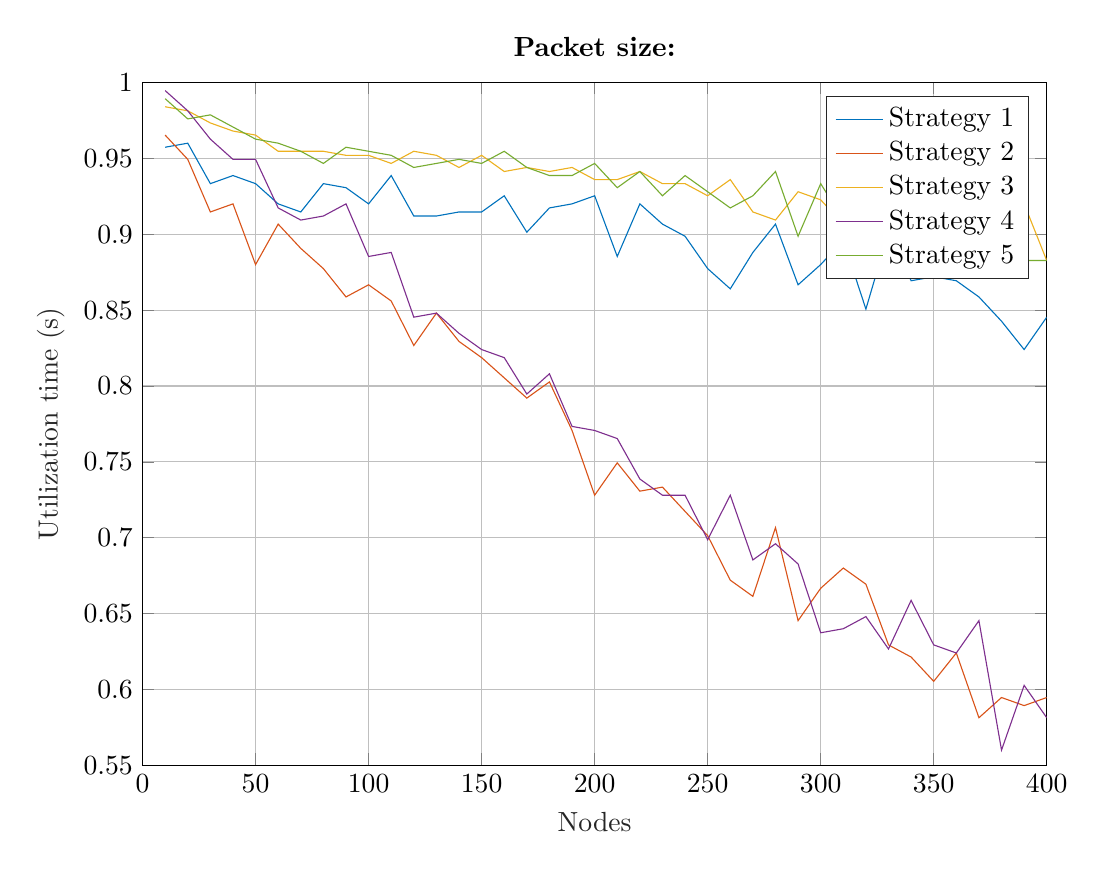
\begin{tikzpicture}

\begin{axis}[%
width=4.521in,
height=3.414in,
at={(0.758in,0.481in)},
scale only axis,
xmin=0,
xmax=400,
xlabel style={font=\color{white!15!black}},
xlabel={Nodes},
ymin=0.55,
ymax=1,
ylabel style={font=\color{white!15!black}},
ylabel={Utilization time (s)},
axis background/.style={fill=white},
title style={font=\bfseries},
title={Packet size:},
xmajorgrids,
ymajorgrids,
legend style={legend cell align=left, align=left, draw=white!15!black}
]
\addplot [color=mycolor1]
  table[row sep=crcr]{%
10	0.957333333333333\\
20	0.96\\
30	0.933333333333333\\
40	0.938666666666666\\
50	0.933333333333333\\
60	0.919999999999999\\
70	0.914666666666666\\
80	0.933333333333333\\
90	0.930666666666666\\
100	0.919999999999999\\
110	0.938666666666666\\
120	0.911999999999999\\
130	0.911999999999999\\
140	0.914666666666666\\
150	0.914666666666666\\
160	0.925333333333333\\
170	0.901333333333333\\
180	0.917333333333333\\
190	0.919999999999999\\
200	0.925333333333333\\
210	0.885333333333332\\
220	0.919999999999999\\
230	0.906666666666666\\
240	0.898666666666666\\
250	0.877333333333332\\
260	0.863999999999999\\
270	0.887999999999999\\
280	0.906666666666666\\
290	0.866666666666666\\
300	0.879999999999999\\
310	0.895999999999999\\
320	0.850666666666665\\
330	0.901333333333333\\
340	0.869333333333332\\
350	0.871999999999999\\
360	0.869333333333332\\
370	0.858666666666666\\
380	0.842666666666665\\
390	0.823999999999999\\
400	0.845333333333332\\
};
\addlegendentry{Strategy 1}

\addplot [color=mycolor2]
  table[row sep=crcr]{%
10	0.965333333333333\\
20	0.949333333333333\\
30	0.914666666666666\\
40	0.919999999999999\\
50	0.879999999999999\\
60	0.906666666666666\\
70	0.890666666666666\\
80	0.877333333333332\\
90	0.858666666666666\\
100	0.866666666666666\\
110	0.855999999999999\\
120	0.826666666666665\\
130	0.847999999999999\\
140	0.829333333333332\\
150	0.818666666666665\\
160	0.805333333333332\\
170	0.791999999999998\\
180	0.802666666666665\\
190	0.770666666666665\\
200	0.727999999999998\\
210	0.749333333333331\\
220	0.730666666666664\\
230	0.733333333333331\\
240	0.717333333333331\\
250	0.701333333333331\\
260	0.671999999999997\\
270	0.661333333333331\\
280	0.706666666666664\\
290	0.64533333333333\\
300	0.666666666666664\\
310	0.679999999999997\\
320	0.669333333333331\\
330	0.62933333333333\\
340	0.62133333333333\\
350	0.60533333333333\\
360	0.623999999999997\\
370	0.58133333333333\\
380	0.594666666666663\\
390	0.58933333333333\\
400	0.594666666666663\\
};
\addlegendentry{Strategy 2}

\addplot [color=mycolor3]
  table[row sep=crcr]{%
10	0.984\\
20	0.981333333333333\\
30	0.973333333333333\\
40	0.968\\
50	0.965333333333333\\
60	0.954666666666666\\
70	0.954666666666666\\
80	0.954666666666666\\
90	0.952\\
100	0.952\\
110	0.946666666666666\\
120	0.954666666666666\\
130	0.952\\
140	0.944\\
150	0.952\\
160	0.941333333333333\\
170	0.944\\
180	0.941333333333333\\
190	0.944\\
200	0.936\\
210	0.936\\
220	0.941333333333333\\
230	0.933333333333333\\
240	0.933333333333333\\
250	0.925333333333333\\
260	0.936\\
270	0.914666666666666\\
280	0.909333333333333\\
290	0.927999999999999\\
300	0.922666666666666\\
310	0.906666666666666\\
320	0.911999999999999\\
330	0.919999999999999\\
340	0.925333333333333\\
350	0.914666666666666\\
360	0.909333333333333\\
370	0.927999999999999\\
380	0.893333333333333\\
390	0.919999999999999\\
400	0.882666666666666\\
};
\addlegendentry{Strategy 3}

\addplot [color=mycolor4]
  table[row sep=crcr]{%
10	0.994666666666667\\
20	0.981333333333333\\
30	0.962666666666666\\
40	0.949333333333333\\
50	0.949333333333333\\
60	0.917333333333333\\
70	0.909333333333333\\
80	0.911999999999999\\
90	0.919999999999999\\
100	0.885333333333332\\
110	0.887999999999999\\
120	0.845333333333332\\
130	0.847999999999999\\
140	0.834666666666665\\
150	0.823999999999999\\
160	0.818666666666665\\
170	0.794666666666665\\
180	0.807999999999998\\
190	0.773333333333332\\
200	0.770666666666665\\
210	0.765333333333331\\
220	0.738666666666665\\
230	0.727999999999998\\
240	0.727999999999998\\
250	0.698666666666664\\
260	0.727999999999998\\
270	0.685333333333331\\
280	0.695999999999998\\
290	0.682666666666664\\
300	0.63733333333333\\
310	0.639999999999997\\
320	0.647999999999997\\
330	0.626666666666664\\
340	0.658666666666664\\
350	0.62933333333333\\
360	0.623999999999997\\
370	0.64533333333333\\
380	0.559999999999996\\
390	0.602666666666663\\
400	0.58133333333333\\
};
\addlegendentry{Strategy 4}

\addplot [color=mycolor5]
  table[row sep=crcr]{%
10	0.989333333333333\\
20	0.976\\
30	0.978666666666667\\
40	0.970666666666667\\
50	0.962666666666666\\
60	0.96\\
70	0.954666666666666\\
80	0.946666666666666\\
90	0.957333333333333\\
100	0.954666666666666\\
110	0.952\\
120	0.944\\
130	0.946666666666666\\
140	0.949333333333333\\
150	0.946666666666666\\
160	0.954666666666666\\
170	0.944\\
180	0.938666666666666\\
190	0.938666666666666\\
200	0.946666666666666\\
210	0.930666666666666\\
220	0.941333333333333\\
230	0.925333333333333\\
240	0.938666666666666\\
250	0.927999999999999\\
260	0.917333333333333\\
270	0.925333333333333\\
280	0.941333333333333\\
290	0.898666666666666\\
300	0.933333333333333\\
310	0.909333333333333\\
320	0.922666666666666\\
330	0.901333333333333\\
340	0.911999999999999\\
350	0.911999999999999\\
360	0.901333333333333\\
370	0.914666666666666\\
380	0.925333333333333\\
390	0.882666666666666\\
400	0.882666666666666\\
};
\addlegendentry{Strategy 5}

\end{axis}
\end{tikzpicture}%
        \caption{Packet size = 16000 bits}
    \end{subfigure}


    \begin{subfigure}{0.45\linewidth}
        \centering
        % This file was created by matlab2tikz.
%
%The latest updates can be retrieved from
%  http://www.mathworks.com/matlabcentral/fileexchange/22022-matlab2tikz-matlab2tikz
%where you can also make suggestions and rate matlab2tikz.
%
\definecolor{mycolor1}{rgb}{0.00000,0.44700,0.74100}%
\definecolor{mycolor2}{rgb}{0.85000,0.32500,0.09800}%
\definecolor{mycolor3}{rgb}{0.92900,0.69400,0.12500}%
\definecolor{mycolor4}{rgb}{0.49400,0.18400,0.55600}%
\definecolor{mycolor5}{rgb}{0.46600,0.67400,0.18800}%
%
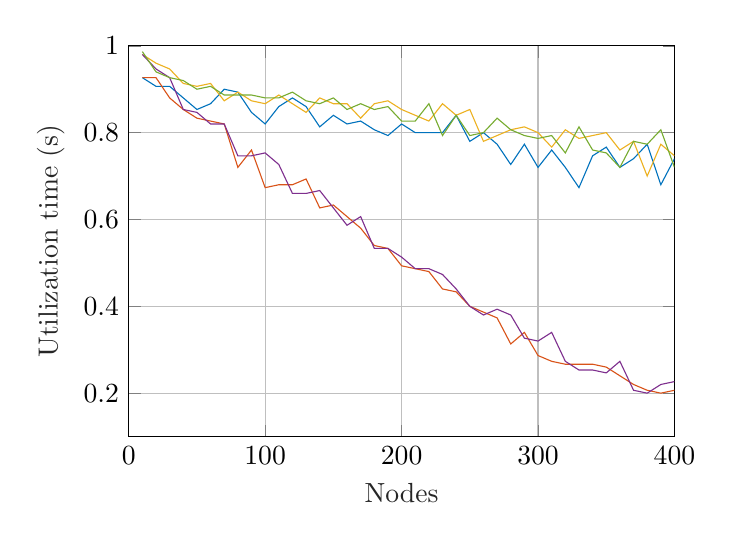
\begin{tikzpicture}

\begin{axis}[%
width=4.521in,
height=3.414in,
at={(0.758in,0.481in)},
scale =0.7,
xmin=0,
xmax=400,
xlabel style={font=\color{white!15!black}},
xlabel={Nodes},
ymin=0.1,
ymax=1,
ylabel style={font=\color{white!15!black}},
ylabel={Utilization time (s)},
axis background/.style={fill=white},
title style={font=\bfseries},
title={},
xmajorgrids,
ymajorgrids,
%legend style={at={(0,0)},anchor=south west}
]
\addplot [color=mycolor1]
  table[row sep=crcr]{%
10	0.926666666666667\\
20	0.906666666666666\\
30	0.906666666666666\\
40	0.88\\
50	0.853333333333333\\
60	0.866666666666666\\
70	0.9\\
80	0.893333333333333\\
90	0.846666666666666\\
100	0.819999999999999\\
110	0.86\\
120	0.88\\
130	0.86\\
140	0.813333333333333\\
150	0.84\\
160	0.819999999999999\\
170	0.826666666666666\\
180	0.806666666666666\\
190	0.793333333333333\\
200	0.819999999999999\\
210	0.799999999999999\\
220	0.799999999999999\\
230	0.799999999999999\\
240	0.84\\
250	0.779999999999999\\
260	0.799999999999999\\
270	0.773333333333333\\
280	0.726666666666666\\
290	0.773333333333333\\
300	0.719999999999999\\
310	0.759999999999999\\
320	0.719999999999999\\
330	0.673333333333332\\
340	0.746666666666666\\
350	0.766666666666666\\
360	0.719999999999999\\
370	0.739999999999999\\
380	0.773333333333333\\
390	0.679999999999999\\
400	0.739999999999999\\
};
%\addlegendentry{Strategy 1}

\addplot [color=mycolor2]
  table[row sep=crcr]{%
10	0.926666666666667\\
20	0.926666666666667\\
30	0.88\\
40	0.853333333333333\\
50	0.833333333333333\\
60	0.826666666666666\\
70	0.819999999999999\\
80	0.719999999999999\\
90	0.759999999999999\\
100	0.673333333333332\\
110	0.679999999999999\\
120	0.679999999999999\\
130	0.693333333333332\\
140	0.626666666666665\\
150	0.633333333333332\\
160	0.606666666666665\\
170	0.579999999999998\\
180	0.539999999999998\\
190	0.533333333333332\\
200	0.493333333333331\\
210	0.486666666666665\\
220	0.479999999999998\\
230	0.439999999999998\\
240	0.433333333333332\\
250	0.399999999999999\\
260	0.386666666666665\\
270	0.373333333333332\\
280	0.313333333333332\\
290	0.339999999999999\\
300	0.286666666666666\\
310	0.273333333333332\\
320	0.266666666666666\\
330	0.266666666666666\\
340	0.266666666666666\\
350	0.259999999999999\\
360	0.239999999999999\\
370	0.219999999999999\\
380	0.206666666666666\\
390	0.199999999999999\\
400	0.206666666666666\\
};
%\addlegendentry{Strategy 2}

\addplot [color=mycolor3]
  table[row sep=crcr]{%
10	0.98\\
20	0.96\\
30	0.946666666666667\\
40	0.913333333333333\\
50	0.906666666666666\\
60	0.913333333333333\\
70	0.873333333333333\\
80	0.893333333333333\\
90	0.873333333333333\\
100	0.866666666666666\\
110	0.886666666666666\\
120	0.866666666666666\\
130	0.846666666666666\\
140	0.88\\
150	0.866666666666666\\
160	0.866666666666666\\
170	0.833333333333333\\
180	0.866666666666666\\
190	0.873333333333333\\
200	0.853333333333333\\
210	0.84\\
220	0.826666666666666\\
230	0.866666666666666\\
240	0.84\\
250	0.853333333333333\\
260	0.779999999999999\\
270	0.793333333333333\\
280	0.806666666666666\\
290	0.813333333333333\\
300	0.799999999999999\\
310	0.766666666666666\\
320	0.806666666666666\\
330	0.786666666666666\\
340	0.793333333333333\\
350	0.799999999999999\\
360	0.759999999999999\\
370	0.779999999999999\\
380	0.699999999999999\\
390	0.773333333333333\\
400	0.746666666666666\\
};
%\addlegendentry{Strategy 3}

\addplot [color=mycolor4]
  table[row sep=crcr]{%
10	0.98\\
20	0.946666666666667\\
30	0.926666666666667\\
40	0.853333333333333\\
50	0.846666666666666\\
60	0.819999999999999\\
70	0.819999999999999\\
80	0.746666666666666\\
90	0.746666666666666\\
100	0.753333333333332\\
110	0.726666666666666\\
120	0.659999999999999\\
130	0.659999999999999\\
140	0.666666666666665\\
150	0.626666666666665\\
160	0.586666666666665\\
170	0.606666666666665\\
180	0.533333333333332\\
190	0.533333333333332\\
200	0.513333333333332\\
210	0.486666666666665\\
220	0.486666666666665\\
230	0.473333333333332\\
240	0.439999999999998\\
250	0.399999999999999\\
260	0.379999999999999\\
270	0.393333333333332\\
280	0.379999999999999\\
290	0.326666666666666\\
300	0.319999999999999\\
310	0.339999999999999\\
320	0.273333333333332\\
330	0.253333333333333\\
340	0.253333333333333\\
350	0.246666666666666\\
360	0.273333333333332\\
370	0.206666666666666\\
380	0.199999999999999\\
390	0.219999999999999\\
400	0.226666666666666\\
};
%\addlegendentry{Strategy 4}

\addplot [color=mycolor5]
  table[row sep=crcr]{%
10	0.986666666666667\\
20	0.94\\
30	0.926666666666667\\
40	0.92\\
50	0.9\\
60	0.906666666666666\\
70	0.886666666666666\\
80	0.886666666666666\\
90	0.886666666666666\\
100	0.88\\
110	0.88\\
120	0.893333333333333\\
130	0.873333333333333\\
140	0.866666666666666\\
150	0.88\\
160	0.853333333333333\\
170	0.866666666666666\\
180	0.853333333333333\\
190	0.86\\
200	0.826666666666666\\
210	0.826666666666666\\
220	0.866666666666666\\
230	0.793333333333333\\
240	0.84\\
250	0.793333333333333\\
260	0.799999999999999\\
270	0.833333333333333\\
280	0.806666666666666\\
290	0.793333333333333\\
300	0.786666666666666\\
310	0.793333333333333\\
320	0.753333333333332\\
330	0.813333333333333\\
340	0.759999999999999\\
350	0.753333333333332\\
360	0.719999999999999\\
370	0.779999999999999\\
380	0.773333333333333\\
390	0.806666666666666\\
400	0.719999999999999\\
};
%\addlegendentry{Strategy 5}

\end{axis}
\end{tikzpicture}%
        \caption{Packet size = 40000 bits}
    \end{subfigure}
    \hfill
    \begin{subfigure}{0.45\linewidth}
        \centering
        % This file was created by matlab2tikz.
%
%The latest updates can be retrieved from
%  http://www.mathworks.com/matlabcentral/fileexchange/22022-matlab2tikz-matlab2tikz
%where you can also make suggestions and rate matlab2tikz.
%
\definecolor{mycolor1}{rgb}{0.00000,0.44700,0.74100}%
\definecolor{mycolor2}{rgb}{0.85000,0.32500,0.09800}%
\definecolor{mycolor3}{rgb}{0.92900,0.69400,0.12500}%
\definecolor{mycolor4}{rgb}{0.49400,0.18400,0.55600}%
\definecolor{mycolor5}{rgb}{0.46600,0.67400,0.18800}%
%
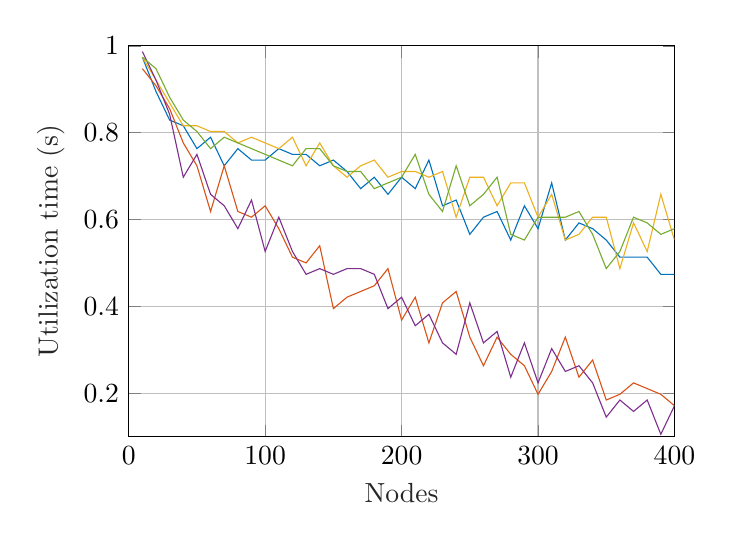
\begin{tikzpicture}

\begin{axis}[%
width=4.521in,
height=3.414in,
at={(0.758in,0.481in)},
scale =0.7,
xmin=0,
xmax=400,
xlabel style={font=\color{white!15!black}},
xlabel={Nodes},
ymin=0.1,
ymax=1,
ylabel style={font=\color{white!15!black}},
ylabel={Utilization time (s)},
axis background/.style={fill=white},
title style={font=\bfseries},
title={},
xmajorgrids,
ymajorgrids,
%legend style={at={(0,0)},anchor=south west}
]
\addplot [color=mycolor1]
  table[row sep=crcr]{%
10	0.973684210526316\\
20	0.894736842105263\\
30	0.828947368421053\\
40	0.815789473684211\\
50	0.763157894736842\\
60	0.789473684210526\\
70	0.723684210526316\\
80	0.763157894736842\\
90	0.736842105263158\\
100	0.736842105263158\\
110	0.763157894736842\\
120	0.75\\
130	0.75\\
140	0.723684210526316\\
150	0.736842105263158\\
160	0.710526315789474\\
170	0.671052631578947\\
180	0.697368421052632\\
190	0.657894736842105\\
200	0.697368421052632\\
210	0.671052631578947\\
220	0.736842105263158\\
230	0.631578947368421\\
240	0.644736842105263\\
250	0.565789473684211\\
260	0.605263157894737\\
270	0.618421052631579\\
280	0.552631578947369\\
290	0.631578947368421\\
300	0.578947368421053\\
310	0.68421052631579\\
320	0.552631578947369\\
330	0.592105263157895\\
340	0.578947368421053\\
350	0.552631578947369\\
360	0.513157894736842\\
370	0.513157894736842\\
380	0.513157894736842\\
390	0.473684210526316\\
400	0.473684210526316\\
};
%\addlegendentry{Strategy 1}

\addplot [color=mycolor2]
  table[row sep=crcr]{%
10	0.947368421052632\\
20	0.907894736842105\\
30	0.855263157894737\\
40	0.776315789473684\\
50	0.723684210526316\\
60	0.618421052631579\\
70	0.723684210526316\\
80	0.618421052631579\\
90	0.605263157894737\\
100	0.631578947368421\\
110	0.578947368421053\\
120	0.513157894736842\\
130	0.5\\
140	0.539473684210527\\
150	0.394736842105263\\
160	0.421052631578948\\
170	0.43421052631579\\
180	0.447368421052632\\
190	0.486842105263158\\
200	0.368421052631579\\
210	0.421052631578948\\
220	0.315789473684211\\
230	0.407894736842105\\
240	0.43421052631579\\
250	0.328947368421053\\
260	0.263157894736842\\
270	0.328947368421053\\
280	0.289473684210527\\
290	0.263157894736842\\
300	0.197368421052632\\
310	0.25\\
320	0.328947368421053\\
330	0.236842105263158\\
340	0.276315789473685\\
350	0.18421052631579\\
360	0.197368421052632\\
370	0.223684210526316\\
380	0.210526315789474\\
390	0.197368421052632\\
400	0.171052631578948\\
};
%\addlegendentry{Strategy 2}

\addplot [color=mycolor3]
  table[row sep=crcr]{%
10	0.973684210526316\\
20	0.921052631578947\\
30	0.868421052631579\\
40	0.815789473684211\\
50	0.815789473684211\\
60	0.802631578947368\\
70	0.802631578947368\\
80	0.776315789473684\\
90	0.789473684210526\\
100	0.776315789473684\\
110	0.763157894736842\\
120	0.789473684210526\\
130	0.723684210526316\\
140	0.776315789473684\\
150	0.723684210526316\\
160	0.697368421052632\\
170	0.723684210526316\\
180	0.736842105263158\\
190	0.697368421052632\\
200	0.710526315789474\\
210	0.710526315789474\\
220	0.697368421052632\\
230	0.710526315789474\\
240	0.605263157894737\\
250	0.697368421052632\\
260	0.697368421052632\\
270	0.631578947368421\\
280	0.68421052631579\\
290	0.68421052631579\\
300	0.605263157894737\\
310	0.657894736842105\\
320	0.552631578947369\\
330	0.565789473684211\\
340	0.605263157894737\\
350	0.605263157894737\\
360	0.486842105263158\\
370	0.592105263157895\\
380	0.526315789473684\\
390	0.657894736842105\\
400	0.552631578947369\\
};
%\addlegendentry{Strategy 3}

\addplot [color=mycolor4]
  table[row sep=crcr]{%
10	0.986842105263158\\
20	0.921052631578947\\
30	0.842105263157895\\
40	0.697368421052632\\
50	0.75\\
60	0.657894736842105\\
70	0.631578947368421\\
80	0.578947368421053\\
90	0.644736842105263\\
100	0.526315789473684\\
110	0.605263157894737\\
120	0.526315789473684\\
130	0.473684210526316\\
140	0.486842105263158\\
150	0.473684210526316\\
160	0.486842105263158\\
170	0.486842105263158\\
180	0.473684210526316\\
190	0.394736842105263\\
200	0.421052631578948\\
210	0.355263157894737\\
220	0.381578947368421\\
230	0.315789473684211\\
240	0.289473684210527\\
250	0.407894736842105\\
260	0.315789473684211\\
270	0.342105263157895\\
280	0.236842105263158\\
290	0.315789473684211\\
300	0.223684210526316\\
310	0.302631578947369\\
320	0.25\\
330	0.263157894736842\\
340	0.223684210526316\\
350	0.144736842105263\\
360	0.18421052631579\\
370	0.157894736842105\\
380	0.18421052631579\\
390	0.105263157894737\\
400	0.171052631578948\\
};
%\addlegendentry{Strategy 4}

\addplot [color=mycolor5]
  table[row sep=crcr]{%
10	0.973684210526316\\
20	0.947368421052632\\
30	0.881578947368421\\
40	0.828947368421053\\
50	0.802631578947368\\
60	0.763157894736842\\
70	0.789473684210526\\
80	0.776315789473684\\
90	0.763157894736842\\
100	0.75\\
110	0.736842105263158\\
120	0.723684210526316\\
130	0.763157894736842\\
140	0.763157894736842\\
150	0.723684210526316\\
160	0.710526315789474\\
170	0.710526315789474\\
180	0.671052631578947\\
190	0.68421052631579\\
200	0.697368421052632\\
210	0.75\\
220	0.657894736842105\\
230	0.618421052631579\\
240	0.723684210526316\\
250	0.631578947368421\\
260	0.657894736842105\\
270	0.697368421052632\\
280	0.565789473684211\\
290	0.552631578947369\\
300	0.605263157894737\\
310	0.605263157894737\\
320	0.605263157894737\\
330	0.618421052631579\\
340	0.565789473684211\\
350	0.486842105263158\\
360	0.526315789473684\\
370	0.605263157894737\\
380	0.592105263157895\\
390	0.565789473684211\\
400	0.578947368421053\\
};
%\addlegendentry{Strategy 5}

\end{axis}
\end{tikzpicture}%
        \caption{Packet size = 80000 bits}
    \end{subfigure}

    \caption{So sánh thời gian gửi thành công gói tin với các kích thước khác nhau và chiến lược khác nhau}
    \label{fig:result}
\end{figure}

Utilization time là thời gian để gói tin được chuyển thành công, hay nói cách khác đây là biến thể hiện khả năng sử dụng kênh một cách hiệu quả của mạng, tức là phần trăm thời gian mà kênh được sử dụng để truyền dữ liệu thành công so với tổng thời gian. Giá trị càng cao thường cho thấy mạng hoạt động hiệu quả hơn trong việc truyền dữ liệu.
